\documentclass[aspectratio=169,11pt]{beamer}
\usepackage[T1]{fontenc}
\usepackage{lmodern}
\usepackage[scaled=0.92]{helvet}
\renewcommand{\familydefault}{\sfdefault}
\usepackage{booktabs,graphicx,tikz,array}
\newcolumntype{L}[1]{>{\raggedright\arraybackslash}p{#1}}
\usetikzlibrary{positioning,arrows.meta,fit,calc}
\definecolor{ink}{HTML}{1B1F24}\definecolor{accent}{HTML}{1F4E79}\definecolor{muted}{HTML}{6B7280}
\definecolor{hair}{HTML}{C9CED6}\definecolor{soft}{HTML}{EEF2F6}
\setbeamersize{text margin left=1.1cm,text margin right=1.1cm}
\setbeamercolor{normal text}{fg=ink}\setbeamercolor{structure}{fg=accent}
\setbeamerfont{frametitle}{series=\bfseries,size=\large}
\setbeamertemplate{navigation symbols}{}
\setbeamertemplate{itemize item}{\raisebox{0.25ex}{\textcolor{accent}{\rule{0.65ex}{0.65ex}}}}
\setbeamertemplate{itemize subitem}{\textcolor{muted}{--}}
\setbeamertemplate{enumerate item}{\textcolor{accent}{\insertenumlabel.}}
\setbeamertemplate{frametitle}{\vspace*{1.0em}{\usebeamerfont{frametitle}\textcolor{ink}{\insertframetitle}}\par\vspace{0.4em}{\color{accent}\hrule height 0.9pt}}
\setbeamertemplate{footline}{\leavevmode\hbox to \paperwidth{\hspace*{1.1cm}\color{muted}\scriptsize
  Multi-Agent LLM Trading on NSE Equities\quad\textbar\quad MTP Final Evaluation\hfill\insertframenumber\,/\,\inserttotalframenumber\hspace*{1.1cm}}\vspace*{0.8em}}
\newenvironment{pts}{\begin{itemize}\setlength{\itemsep}{0.6em}}{\end{itemize}}
\newcommand{\lead}[1]{{\small\bfseries\color{accent}#1}\par\vspace{0.35em}}
\newcommand{\src}[1]{\par\vspace{0.45em}{\scriptsize\color{muted}#1\par}}
\tikzset{box/.style={draw=accent,line width=0.6pt,rounded corners=1.5pt,fill=soft,align=center,font=\footnotesize,inner sep=5pt,minimum height=0.95cm},
  wide/.style={box,fill=white,text width=12.35cm},
  arr/.style={-{Stealth[length=5pt]},line width=0.6pt,color=muted},
  lab/.style={font=\scriptsize,color=muted}}
\begin{document}
{\setbeamertemplate{footline}{}
\begin{frame}[plain,noframenumbering]
\vspace*{1.6cm}
{\color{accent}\rule{2.2cm}{2.2pt}}\par\vspace{0.9em}
{\LARGE\bfseries A Multi-Agent LLM Framework for Explainable\\[0.25em]Algorithmic Trading on NSE-Listed Equities}\par\vspace{0.9em}
{\large\color{muted}M.Tech Project, Final Evaluation}\par\vspace{2.0em}
\begin{tabular}{@{}ll@{}}
\textcolor{muted}{Presented by} & \textbf{Vipluv} (22MF3IM22)\\[0.25em]
\textcolor{muted}{Supervisor} & Prof.\ S.\ P.\ Sarmah\\[0.25em]
\textcolor{muted}{Department} & Industrial \& Systems Engineering, IIT Kharagpur\\[0.25em]
\textcolor{muted}{Date} & November 2026
\end{tabular}
\end{frame}}

\begin{frame}{Outline}

\vspace{0.4em}
\begin{enumerate}\setlength{\itemsep}{0.75em}
\item Motivation and objectives
\item System design
\item Evaluation protocol
\item Work done since the mid-semester evaluation
\item Results: core and extended universe
\item Explainability evaluation
\item Conclusions, limitations and future work
\end{enumerate}
\end{frame}

\begin{frame}{Motivation\hfill{\normalfont\footnotesize\color{muted}Introduction}}

\begin{pts}
\item Most stock-prediction models output a score without a reason, are tested on US indices, and ignore transaction costs.
\item A trading desk works differently: technical, fundamental, sentiment and risk specialists give separate views, and these are argued out before a trade.
\item Recent papers copy this structure with LLM agents, but there is little evidence on Indian equities under Indian costs.
\end{pts}
\vspace{0.9em}
\lead{Objective}
Build an explainable multi-agent decision-support system for NSE stocks, and test it out-of-sample with the full Indian delivery cost structure.
\end{frame}

\begin{frame}{Work completed\hfill{\normalfont\footnotesize\color{muted}Introduction}}
\begin{columns}[t]\begin{column}{0.46\textwidth}
\lead{Up to mid-semester}
\begin{itemize}\setlength{\itemsep}{0.4em}\small
\item Technical agent (LSTM with temporal attention)
\item LLM sentiment agent on news headlines
\item Regime agent
\item Bull/bear debate
\item Deterministic risk manager
\item Cost-aware backtester and baselines
\end{itemize}\end{column}\begin{column}{0.51\textwidth}
\lead{Since mid-semester (November plan)}
\begin{itemize}\setlength{\itemsep}{0.4em}\small
\item Larger LLM (Qwen2.5-3B) compared with 1.5B
\item Universe extended from 10 to 30 stocks, longer period
\item Sentiment study around earnings days
\item Point-in-time fundamentals agent
\item Cost-aware sizing and no-trade band
\item Full ablation re-run
\item Explainability evaluation
\end{itemize}\end{column}\end{columns}
\end{frame}

\begin{frame}{System architecture\hfill{\normalfont\footnotesize\color{muted}System design}}

\centering
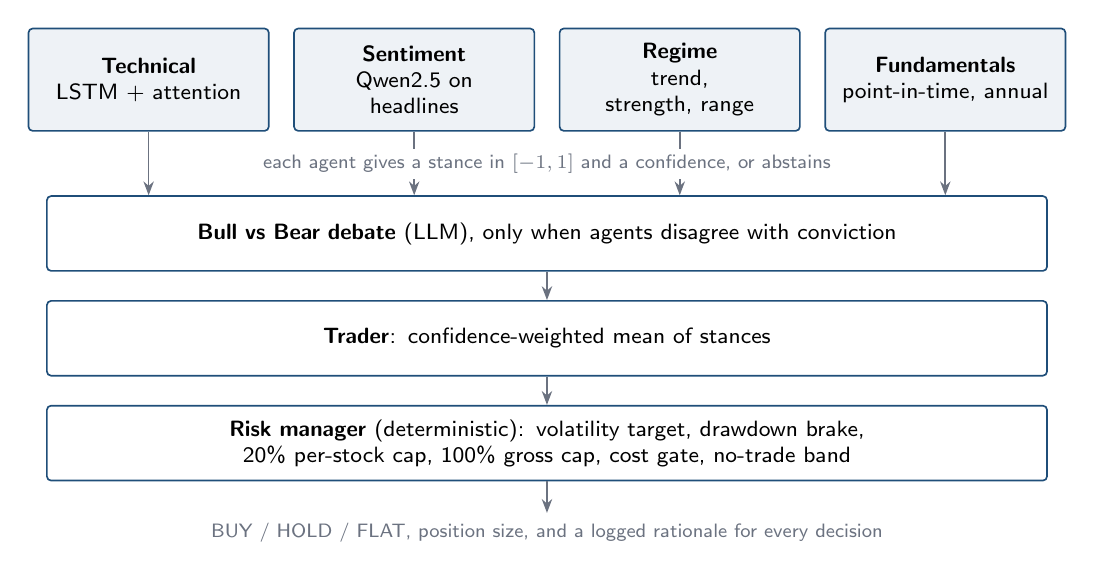
\begin{tikzpicture}[node distance=0.36cm and 0.3cm]
\node[box,text width=2.7cm,minimum height=1.3cm] (t) {\textbf{Technical}\\LSTM + attention};
\node[box,text width=2.7cm,minimum height=1.3cm,right=of t] (s) {\textbf{Sentiment}\\Qwen2.5 on headlines};
\node[box,text width=2.7cm,minimum height=1.3cm,right=of s] (r) {\textbf{Regime}\\trend, strength, range};
\node[box,text width=2.7cm,minimum height=1.3cm,right=of r] (f) {\textbf{Fundamentals}\\point-in-time, annual};
\node[fit=(t)(f),inner sep=0pt] (agents) {};
\node[wide,below=0.8cm of agents] (d) {\textbf{Bull vs Bear debate} (LLM), only when agents disagree with conviction};
\node[wide,below=of d] (tr) {\textbf{Trader}: confidence-weighted mean of stances};
\node[wide,below=of tr] (rm) {\textbf{Risk manager} (deterministic): volatility target, drawdown brake,\\20\% per-stock cap, 100\% gross cap, cost gate, no-trade band};
\node[lab,below=0.4cm of rm] (out) {BUY / HOLD / FLAT, position size, and a logged rationale for every decision};
\foreach \a in {t,s,r,f} \draw[arr] (\a.south) -- (\a.south |- d.north);
\draw[arr] (d) -- (tr); \draw[arr] (tr) -- (rm); \draw[arr] (rm) -- (out);
\node[lab,fill=white,inner sep=2pt] at ($(agents.south)!0.5!(d.north)$) {each agent gives a stance in $[-1,1]$ and a confidence, or abstains};
\end{tikzpicture}
\end{frame}

\begin{frame}{Evaluation protocol\hfill{\normalfont\footnotesize\color{muted}Evaluation}}

\small\renewcommand{\arraystretch}{1.55}
\begin{tabular}{@{}L{3.0cm}L{10.0cm}@{}}
\toprule
\textcolor{muted}{Validation} & Purged, embargoed walk-forward: 3 years train, 6 months test, 10-day embargo, 16 folds\\
\textcolor{muted}{Sample} & 19,110 out-of-sample decisions, 2018-12-07 to 2026-08-27\\
\textcolor{muted}{Execution} & Decide at close of day $t$, trade at open of day $t+1$\\
\textcolor{muted}{Costs} & STT 0.1\% each side, stamp duty, NSE/SEBI charges, GST, 5 bps slippage: about \textbf{32 bps per round trip}\\
\textcolor{muted}{Statistics} & Block-bootstrap confidence intervals, Holm correction over all configurations, Deflated Sharpe Ratio\\
\textcolor{muted}{New parameters} & Fixed before the run: band 0.05, conviction floor 0.10\\
\textcolor{muted}{Reproducibility} & Mid-sem configurations reproduce within 0.004 Sharpe; Buy\&Hold moved 0.58 to 0.59 after a price-snapshot correction\\
\bottomrule
\end{tabular}
\end{frame}

\begin{frame}{Fundamentals agent (point-in-time)\hfill{\normalfont\footnotesize\color{muted}Work since mid-sem}}

\begin{pts}
\item Data: annual P\&L and balance sheet for 30 stocks, FY2015 to FY2026.
\item A report is used only from FY end + 61 days, following the 60-day filing deadline in SEBI LODR Reg.\ 33. This avoids look-ahead.
\item Features: profit growth, revenue growth, ROE and change in ROE, z-scored across peers on each date.
\item Fiscal-year changes are handled separately (HCLTECH 9-month FY2016, NESTLEIND 15-month FY2024).
\item Limitations: figures are restated, not as first published; no valuation ratios such as P/E.
\end{pts}
\src{Sample rationale: ``FY report Mar 2021 (public since 2021-05-31): return on equity +38.2\% is the strongest vs peers (z +2.1)''}
\end{frame}

\begin{frame}{Sentiment around earnings announcements\hfill{\normalfont\footnotesize\color{muted}Work since mid-sem}}
\begin{columns}[c]\begin{column}{0.55\textwidth}\begin{itemize}\setlength{\itemsep}{0.3em}\footnotesize
\item About 10\% of headlines are results news. These days do move more: mean absolute next-day return 133 vs 126 bps (p = 0.029).
\item On the full corpus, tone does not predict direction at 1 or 5 days.
\item Raw tone on earnings headlines shows a reversal (IC about $-0.085$), but it disappears after debiasing and is smaller than costs.
\end{itemize}\vspace{0.3em}{\scriptsize\setlength{\tabcolsep}{4pt}\renewcommand{\arraystretch}{1.12}\begin{tabular}{@{}llrrrr@{}}\toprule
\textcolor{muted}{Model} & \textcolor{muted}{Subset} & \textcolor{muted}{n} & \textcolor{muted}{IC} & \textcolor{muted}{Holm p} & \textcolor{muted}{Hit rate} \\\midrule
Qwen2.5-1.5B & all news & 15190 & +0.00 & 1.00 & 50.1\% \\
Qwen2.5-1.5B & earnings & 1803 & -0.03 & 1.00 & 48.7\% \\
Qwen2.5-1.5B & non-earnings & 13387 & +0.01 & 1.00 & 50.2\% \\
Qwen2.5-3B & all news & 6480 & -0.03 & 0.82 & 49.2\% \\
Qwen2.5-3B & earnings & 1803 & -0.06 & 0.36 & 47.9\% \\
Qwen2.5-3B & non-earnings & 4677 & -0.01 & 1.00 & 49.7\% \\
\bottomrule\end{tabular}}\src{IC of debiased tone against the next-day return.}\end{column}\begin{column}{0.42\textwidth}\centering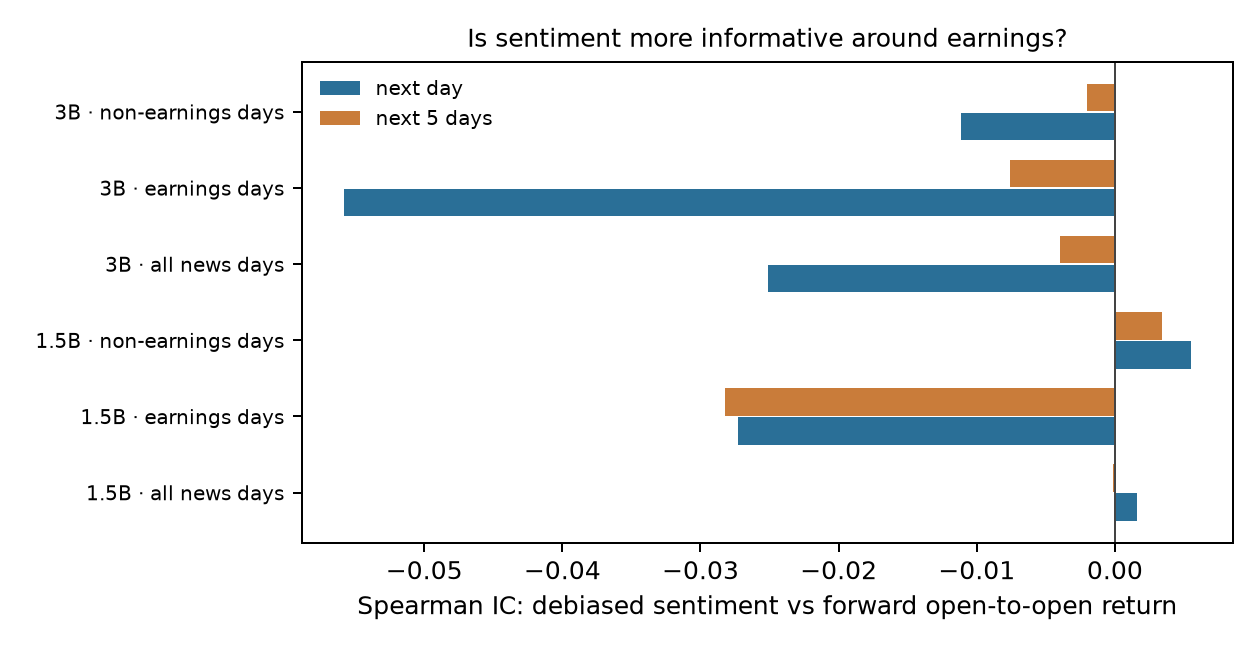
\includegraphics[height=0.66\textheight,width=\linewidth,keepaspectratio]{earnings_ic.png}\end{column}\end{columns}
\end{frame}

\begin{frame}{Effect of a larger LLM: Qwen2.5-3B vs 1.5B\hfill{\normalfont\footnotesize\color{muted}Work since mid-sem}}
\begin{columns}[c]\begin{column}{0.50\textwidth}\begin{itemize}\setlength{\itemsep}{0.5em}\small\item The 1.5B model labels Good 3.31 times as often as Bad on the full corpus. This is a bias of the model, not of the news.\item On the same 10,240 headlines and prompt, the two models agree on 60.3\% of labels ($\kappa$ = 0.39).\item The 3B model is much less bullish and answers Unknown about twice as often.\end{itemize}\vspace{0.5em}{\small\setlength{\tabcolsep}{4pt}\renewcommand{\arraystretch}{1.12}\begin{tabular}{@{}lrrr@{}}\toprule
\textcolor{muted}{Model} & \textcolor{muted}{IC} & \textcolor{muted}{Holm p} & \textcolor{muted}{Hit rate} \\\midrule
Qwen2.5-1.5B & -0.02 & 0.13 & 48.4\% \\
Qwen2.5-3B & -0.03 & 0.09 & 49.2\% \\
\bottomrule\end{tabular}}\src{Neither model gives a usable long-only signal.}\end{column}\begin{column}{0.47\textwidth}\centering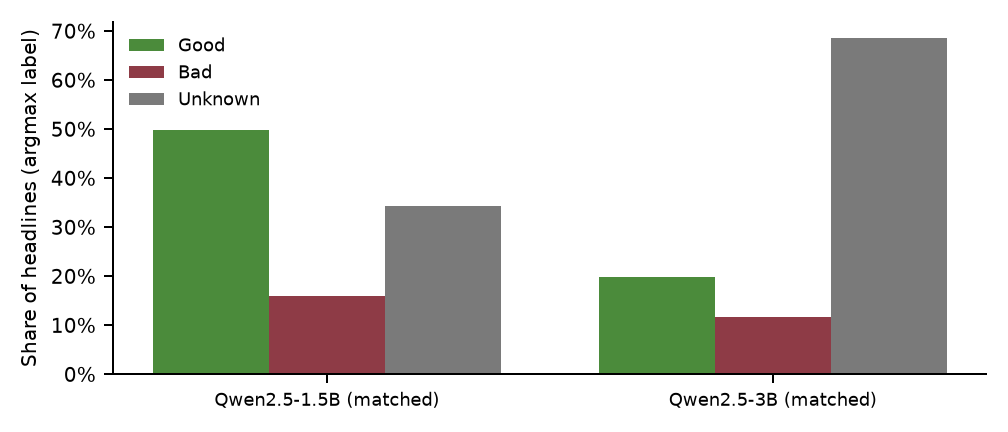
\includegraphics[height=0.62\textheight,width=\linewidth,keepaspectratio]{llm_labels.png}\end{column}\end{columns}
\end{frame}

\begin{frame}{Ablation results: core universe, net of costs\hfill{\normalfont\footnotesize\color{muted}Results}}
\vspace{-0.2em}{\centering{\scriptsize\setlength{\tabcolsep}{4pt}\renewcommand{\arraystretch}{1.12}\begin{tabular}{@{}lrrrrrr@{}}\toprule
\textcolor{muted}{Strategy} & \textcolor{muted}{Net Sharpe} & \textcolor{muted}{Gross Sharpe} & \textcolor{muted}{Max DD} & \textcolor{muted}{Turnover/yr} & \textcolor{muted}{Exposure} & \textcolor{muted}{Holm p} \\\midrule
\textbf{Buy\&Hold} & \textbf{0.59} & \textbf{0.59} & \textbf{-38.6\%} & \textbf{0x} & \textbf{100\%} & \textbf{--} \\
RSI(14) & 0.43 & 0.47 & -39.8\% & 4x & 60\% & 0.82 \\
Tech+Regime & 0.35 & 0.58 & -20.7\% & 20x & 86\% & 0.82 \\
Regime+Fund+Band & 0.28 & 0.47 & -22.2\% & 16x & 84\% & 0.60 \\
Tech+Regime+Fund & 0.24 & 0.50 & -23.2\% & 23x & 88\% & 0.59 \\
Regime+Fund & 0.21 & 0.48 & -23.2\% & 24x & 88\% & 0.59 \\
Tech+Sent+Regime & 0.17 & 0.66 & -25.0\% & 43x & 90\% & 0.41 \\
All4+Debate(conviction) & 0.14 & 0.60 & -24.7\% & 43x & 93\% & 0.09 \\
Full+Debate(conviction) & 0.14 & 0.62 & -27.2\% & 44x & 91\% & 0.21 \\
Tech+Regime+Fund+CostAware+Band & 0.14 & 0.37 & -5.3\% & 5x & 7\% & 0.82 \\
Tech+Sent+Regime+Fund & 0.04 & 0.59 & -25.0\% & 49x & 91\% & 0.14 \\
MACD & 0.02 & 0.46 & -29.9\% & 43x & 78\% & 0.39 \\
KDJ+RSI & -0.34 & 0.24 & -39.3\% & 51x & 34\% & 0.01 \\
Tech-only & -0.41 & -0.27 & -25.4\% & 5x & 16\% & 0.09 \\
All4+CostAware+Band & -0.52 & 0.20 & -5.1\% & 14x & 7\% & 0.21 \\
MeanReversion & -1.41 & 0.68 & -79.6\% & 223x & 76\% & 0.00 \\
\bottomrule\end{tabular}}\par}\src{10 stocks. Sharpe is annualised, in excess of a 6\% risk-free rate. Holm p: paired test against Buy\&Hold.}
\end{frame}

\begin{frame}{Net Sharpe with 95\% confidence intervals\hfill{\normalfont\footnotesize\color{muted}Results}}
\begin{columns}[c]\begin{column}{0.60\textwidth}\centering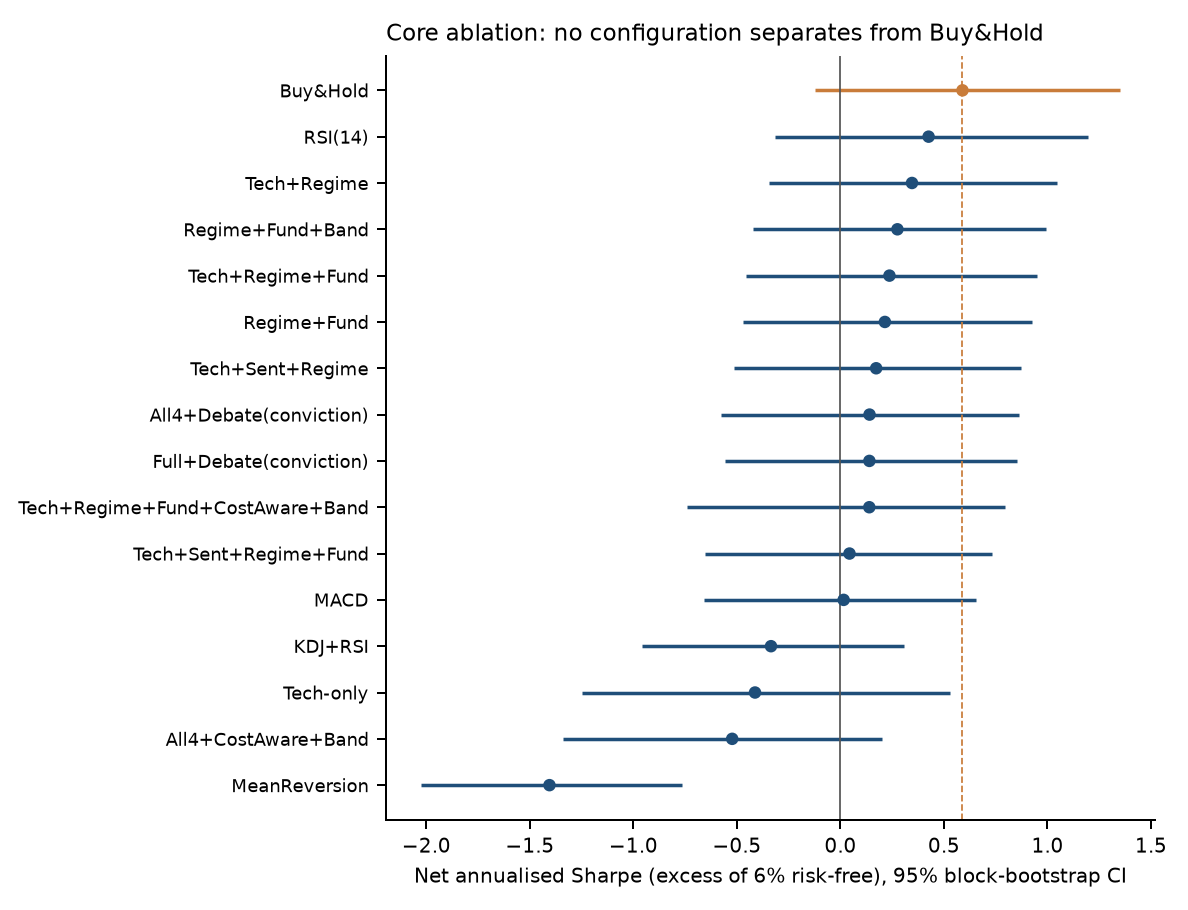
\includegraphics[height=0.76\textheight,width=\linewidth,keepaspectratio]{forest_core.png}\end{column}\begin{column}{0.37\textwidth}
\begin{itemize}\setlength{\itemsep}{0.7em}\small
\item Every interval overlaps Buy\&Hold (0.59).
\item Best agent configuration: Tech+Regime at 0.35.
\item No configuration is significantly better after Holm correction.
\item Mean reversion is significantly worse, because of turnover.
\end{itemize}\end{column}\end{columns}
\end{frame}

\begin{frame}{Effect of each component added since mid-sem\hfill{\normalfont\footnotesize\color{muted}Results}}

\small\renewcommand{\arraystretch}{1.7}
\begin{tabular}{@{}L{3.4cm}L{4.4cm}L{5.1cm}@{}}
\toprule
\textcolor{muted}{Component} & \textcolor{muted}{Net Sharpe} & \textcolor{muted}{Observation}\\
\midrule
\textbf{Fundamentals agent} & Tech+Regime 0.35 to 0.24 & Annual rankings add no daily information \\
\textbf{No-trade band} & Regime+Fund 0.21 to 0.28 & Turnover falls from 24x to 16x a year \\
\textbf{Edge-vs-cost gate} & All4+CostAware+Band -0.52 & Few signals clear 32 bps; average exposure only 7\% \\
\textbf{Conviction-gated debate} & 0.14 (3 agents), 0.14 (4 agents) & Debate on 10.5\% of days instead of 97.4\%; result unchanged \\
\bottomrule
\end{tabular}
\src{The no-trade band is the only addition that improves the net result, and it does so by trading less.}
\end{frame}

\begin{frame}{Equity curves and drawdown: core universe\hfill{\normalfont\footnotesize\color{muted}Results}}
\begin{columns}[c]\begin{column}{0.62\textwidth}\centering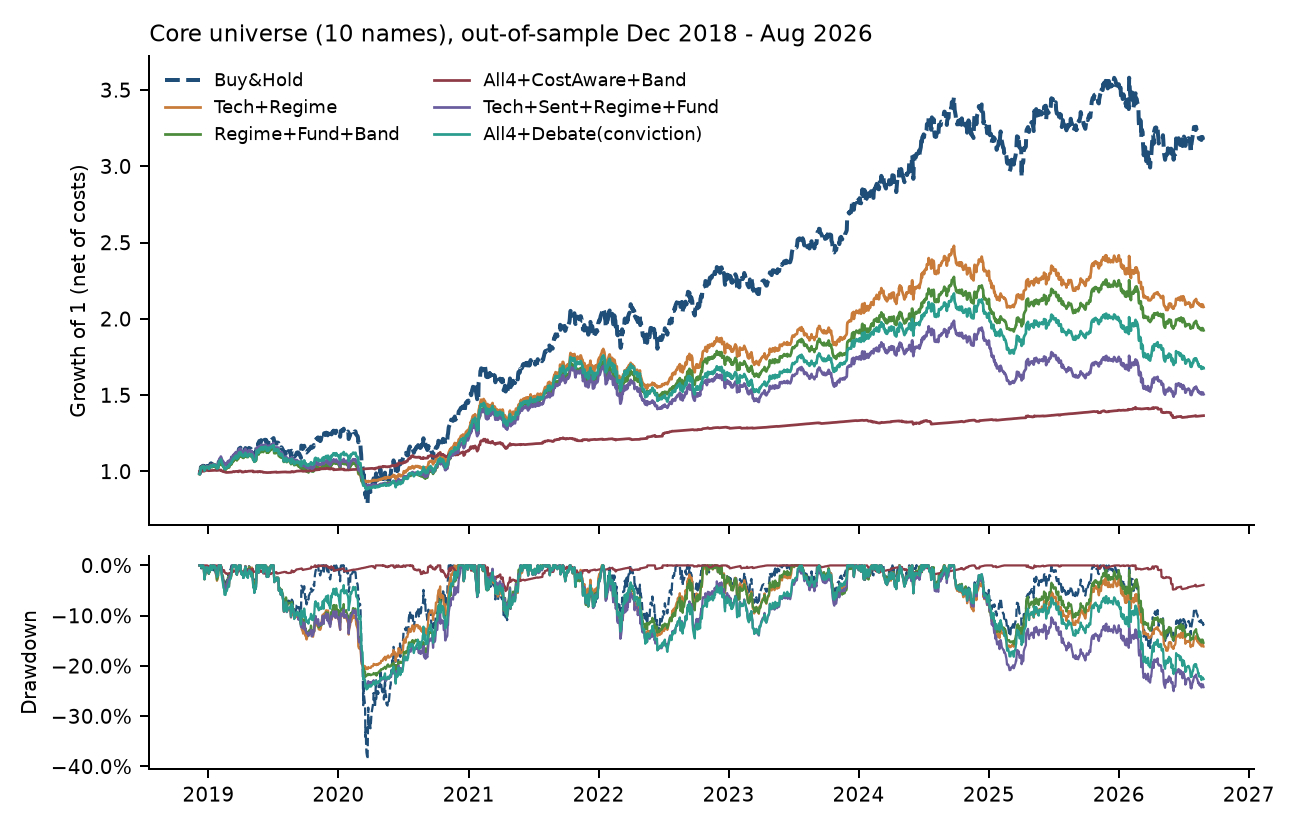
\includegraphics[height=0.76\textheight,width=\linewidth,keepaspectratio]{equity_core.png}\end{column}\begin{column}{0.35\textwidth}
\begin{itemize}\setlength{\itemsep}{0.7em}\small
\item Buy\&Hold ends highest, with a maximum drawdown of -38.6\%.
\item Tech+Regime limits the drawdown to -20.7\%.
\item The risk overlay gives up return in rising markets and protects capital in the 2020 crash.
\end{itemize}\end{column}\end{columns}
\end{frame}

\begin{frame}{Extended universe: 30 stocks, data to 2026-11-04\hfill{\normalfont\footnotesize\color{muted}Results}}
\begin{columns}[c]\begin{column}{0.59\textwidth}{\scriptsize\setlength{\tabcolsep}{4pt}\renewcommand{\arraystretch}{1.12}\begin{tabular}{@{}lrrr@{}}\toprule
\textcolor{muted}{Strategy} & \textcolor{muted}{Sharpe} & \textcolor{muted}{Max DD} & \textcolor{muted}{Turnover} \\\midrule
\textbf{Buy\&Hold} & \textbf{0.74} & \textbf{-34.3\%} & \textbf{0x} \\
RSI(14) & 0.66 & -38.5\% & 9x \\
Regime+Fund+Band & 0.36 & -25.1\% & 16x \\
Tech+Regime & 0.35 & -24.7\% & 29x \\
Tech+Regime+Fund & 0.25 & -27.8\% & 29x \\
Regime+Fund & 0.25 & -27.8\% & 29x \\
MACD & 0.23 & -29.1\% & 70x \\
Tech-only & 0.09 & -7.7\% & 7x \\
Tech+Regime+Fund+CostAware+Band & 0.06 & -17.8\% & 17x \\
KDJ+RSI & -0.92 & -64.2\% & 119x \\
MeanReversion & -1.97 & -91.8\% & 311x \\
\bottomrule\end{tabular}}\src{Same conclusion with three times the stocks and on data not available at mid-sem.}\end{column}\begin{column}{0.38\textwidth}\centering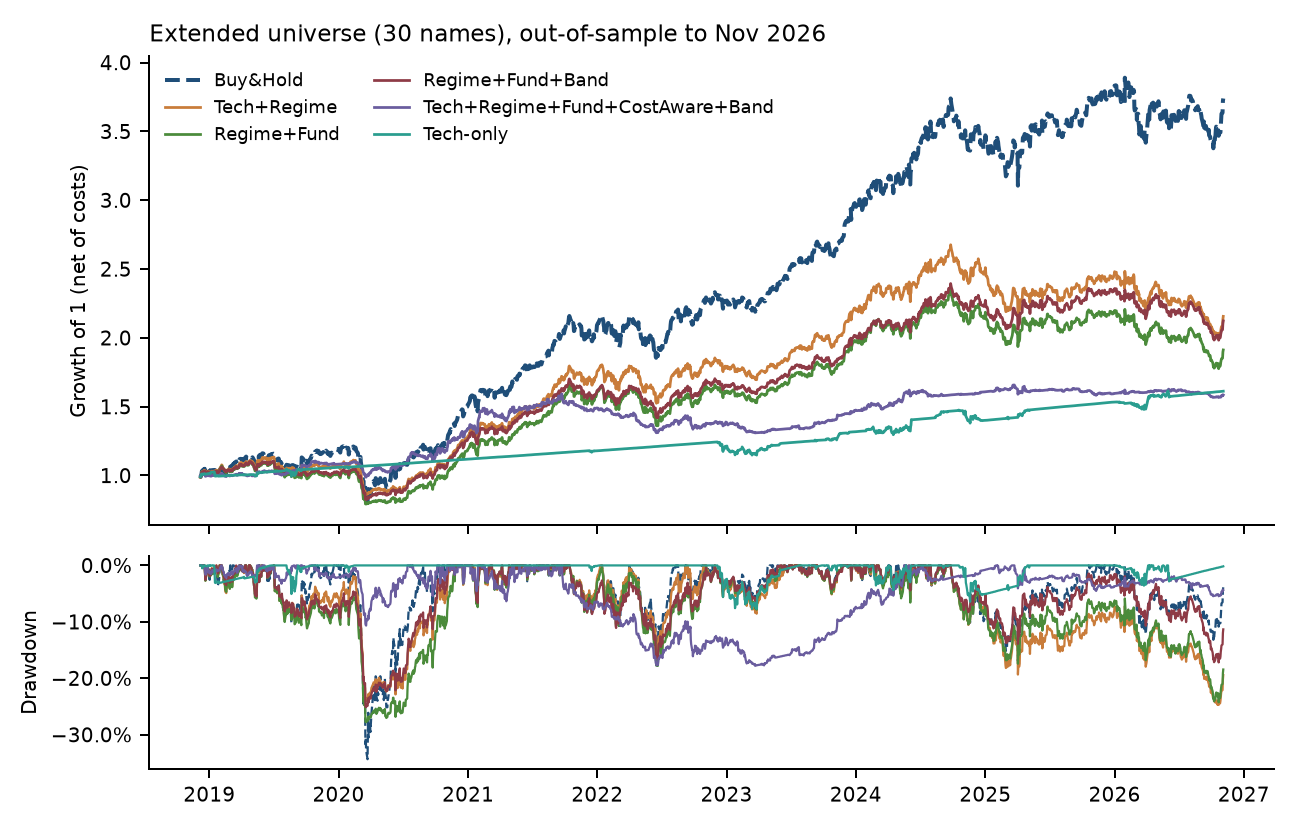
\includegraphics[height=0.70\textheight,width=\linewidth,keepaspectratio]{equity_extended.png}\end{column}\end{columns}
\end{frame}

\begin{frame}{Explainability evaluation\hfill{\normalfont\footnotesize\color{muted}Explainability}}
\begin{columns}[c]\begin{column}{0.58\textwidth}
\footnotesize\setlength{\tabcolsep}{4pt}\renewcommand{\arraystretch}{1.1}
\begin{tabular}{@{}L{2.15cm}L{2.8cm}L{1.85cm}@{}}
\toprule
\textcolor{muted}{Check} & \textcolor{muted}{Question} & \textcolor{muted}{Result}\\
\midrule
\textbf{Provenance} & Does the rationale name the model that produced the number? & 0\% at mid-sem, 100\% after fix\\
\textbf{Integrity} & Do stated stances equal logged stances? & 100\%\\
\textbf{Reconstruction} & Can the score be recomputed from the opinions? & 100\%\\
\textbf{Deletion} & Does removing the top-attributed agent change the decision? & 37\% to 71\% flips (other agent: 0.0\% to 3.4\%)\\
\bottomrule
\end{tabular}
\src{The provenance audit found that all 19,110 mid-sem rationales named PLSTM-TAL for LSTM-TAL predictions.}\end{column}\begin{column}{0.39\textwidth}\centering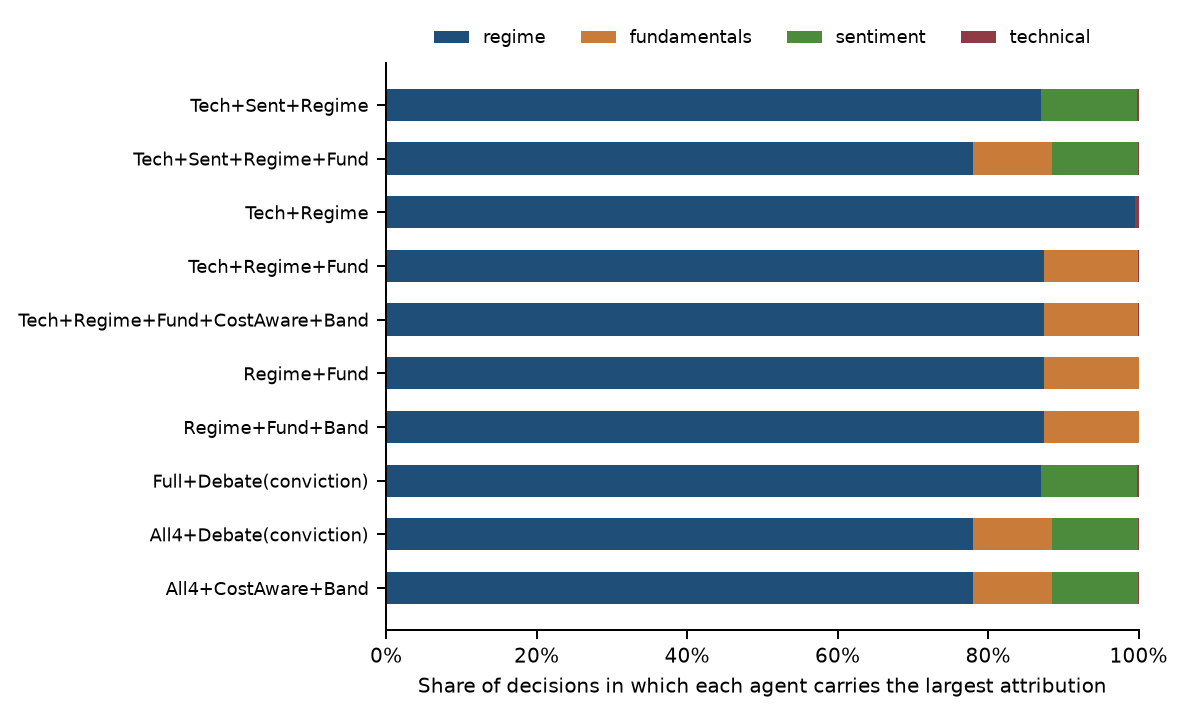
\includegraphics[height=0.62\textheight,width=\linewidth,keepaspectratio]{decisive_agent.png}\src{The regime agent decides most calls: the system behaves as a trend filter.}\end{column}\end{columns}
\end{frame}

\begin{frame}{Accuracy vs explainability\hfill{\normalfont\footnotesize\color{muted}Explainability}}
\begin{columns}[c]\begin{column}{0.58\textwidth}\centering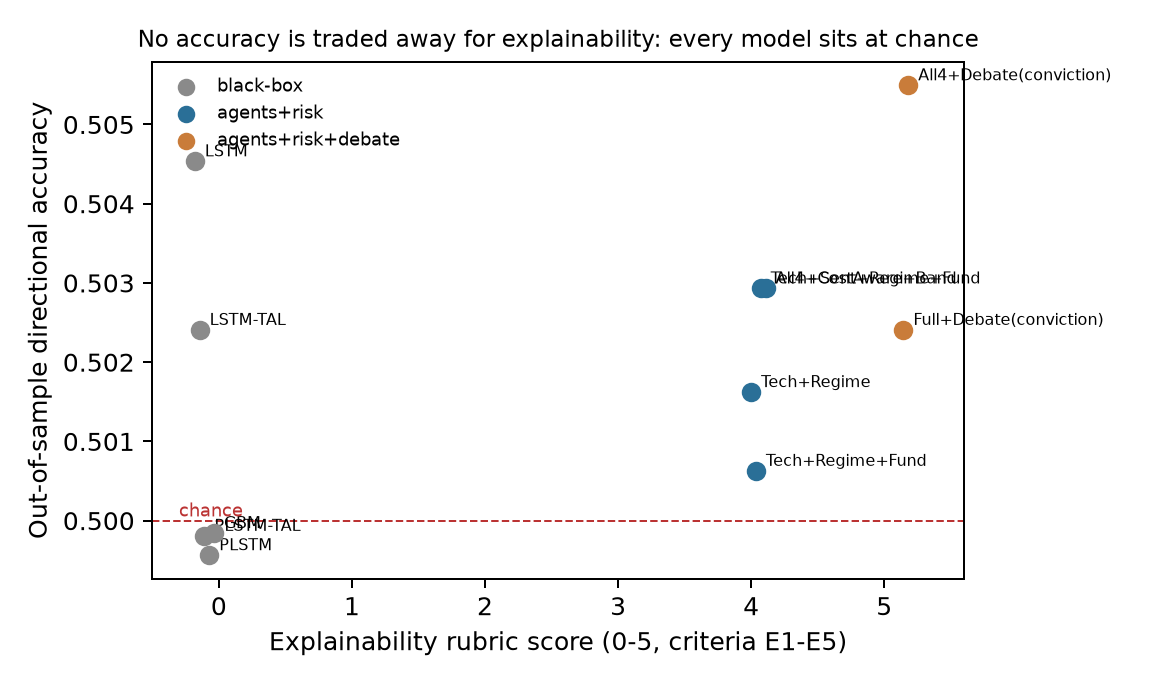
\includegraphics[height=0.74\textheight,width=\linewidth,keepaspectratio]{accuracy_explainability.png}\end{column}\begin{column}{0.39\textwidth}
\begin{itemize}\setlength{\itemsep}{0.7em}\small
\item Black-box models (LSTM variants, GBM) are at chance level.
\item The explainable agent systems are also at chance level.
\item With this little signal, accuracy is limited by the data and not by interpretability.
\item The explainable system has one advantage: it shows why there is no edge.
\end{itemize}\end{column}\end{columns}
\end{frame}

\begin{frame}{Conclusions\hfill{\normalfont\footnotesize\color{muted}Conclusions}}

\begin{pts}
\item The full system was built and tested end to end: four agents, debate, risk manager, cost-aware backtester, a paper-trading demo and over 350 automated tests.
\item \textbf{No configuration beats Buy-and-Hold after Indian transaction costs}, on 10 stocks, on 30 stocks, or on new data.
\item None of the November additions changes this result.
\item The regime-aware risk overlay reduces maximum drawdown by a third to a half.
\item The explanations are faithful by measurement, and the audit found a real provenance bug.
\end{pts}
\end{frame}

\begin{frame}{Limitations and future work\hfill{\normalfont\footnotesize\color{muted}Conclusions}}
\begin{columns}[t]\begin{column}{0.48\textwidth}
\lead{Limitations}
\begin{itemize}\setlength{\itemsep}{0.45em}\small
\item Only open 1.5B and 3B language models
\item Survivorship bias in the stock universe
\item Restated fundamentals
\item Statistical power: detectable Sharpe is about 1.0
\end{itemize}\end{column}\begin{column}{0.49\textwidth}
\lead{Future work}
\begin{itemize}\setlength{\itemsep}{0.45em}\small
\item Event-time and intraday horizons
\item Vendor point-in-time fundamentals
\item Debate with a frontier LLM
\item Market-neutral formulation
\end{itemize}\end{column}\end{columns}
\end{frame}

\begin{frame}{Thank you}
\vspace{1.2em}
{\large Questions?}\par\vspace{2.2em}
\small\renewcommand{\arraystretch}{1.5}
\begin{tabular}{@{}ll@{}}
\textcolor{muted}{Demo (runs in the browser)} & \texttt{vipluv01.github.io/nse-multi-agent-trading}\\
\textcolor{muted}{Code} & \texttt{github.com/Vipluv01/nse-multi-agent-trading}
\end{tabular}
\end{frame}
\end{document}
